\chapter{Conclusions}

\section{Gateway Locations}\label{sec:gateway-locations-conclusions}

This section will evaluate the chosen \acl{LRWGW} locations as described in \Cref{sec:gateway-locations} and give some examples of the ranges that can be achieved with them.
The maps used to show range data were taken from the Advanced Maps feature of \ac{TTNM}~\cite{ttn_mapper_ttn_2023-1}.
Thus, as explained in \Cref{subsec:cleaning-collected-data}, they may contain some inaccuracies and outliers.

\subsection{\acl{GHB}}\label{subsec:ghb-student-dormitory-range-results}

The MikroTik \acl{GW} deployed on top of the \ac{GHB} student dormitory is the \acl{LRWGW} with the highest range in Furtwangen among those deployed during this thesis.
This doesn't come as a surprise, given its exposed location on top of a hill in addition to the height of the building itself.

\begin{figure}[htbp]
    \centering
    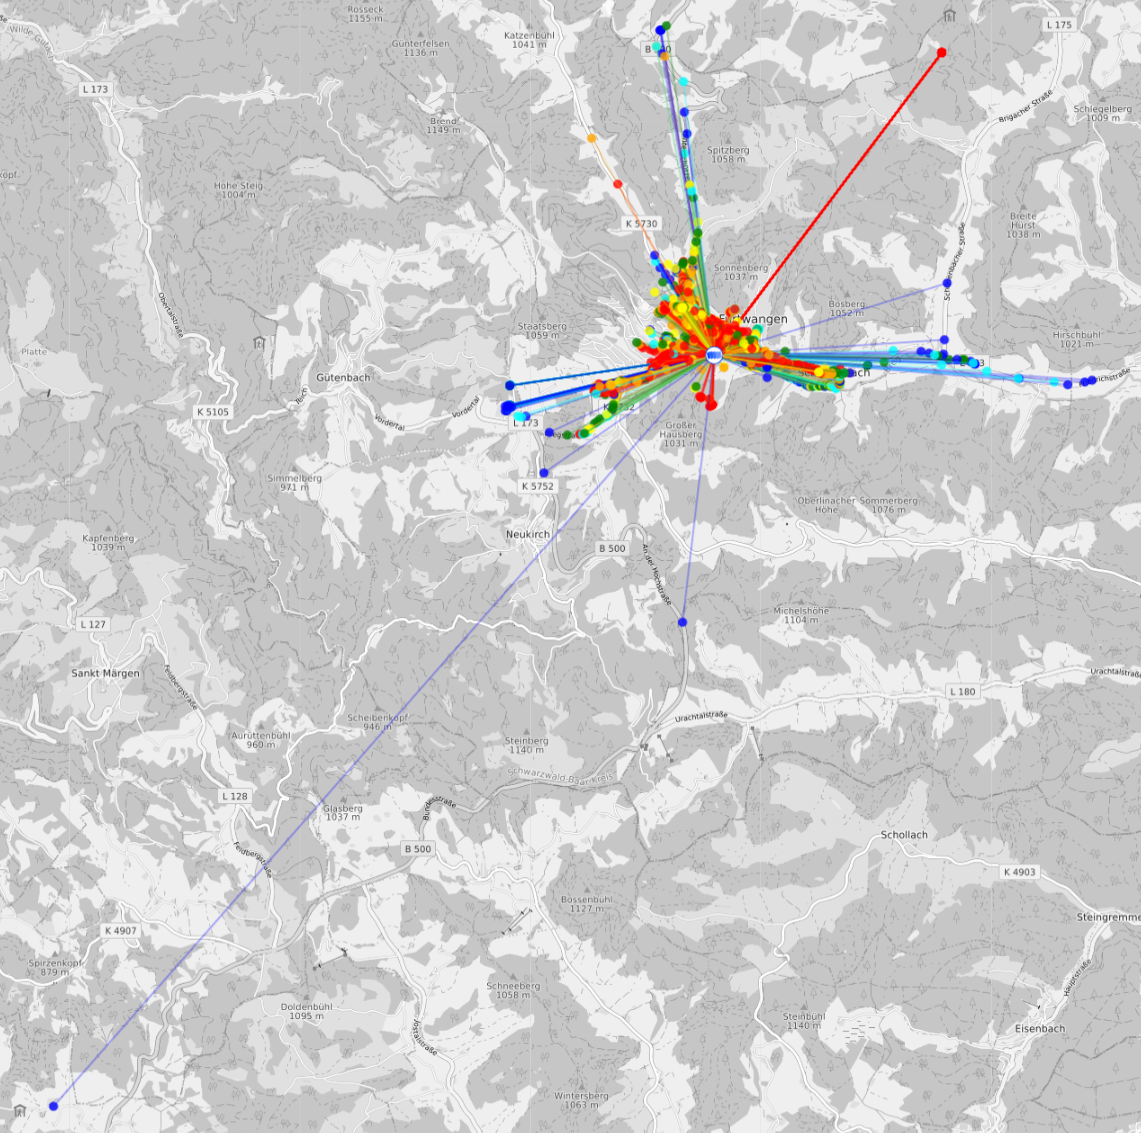
\includegraphics[width=1\textwidth]{pictures/ttn-mapper/gateway-ranges/ghb_mikrotik_gw_range.png}
    \caption[Screenshot of a \acl{TTNM} map showing some data points taken from the \acl{LRWGW} deployed on top of the \acl{GHB}]{
        Screenshot of a \ac{TTNM} map showing some data points taken from the \acl{LRWGW} deployed on top of the \ac{GHB}.
        The data point on the lower left is the maximum range recorded for this \acl{LRWGW} --- \SI{14.2}{\kilo\meter}.
        However, it can be considered an outlier, as the next highest range is \SI{5.3}{\kilo\meter} away from the \acl{LRWGW} (on the far right)~\cite{ttn_mapper_ttn_2023}.
    }\label{pic:ghb_mikrotik_gw_range}
\end{figure}

The maximum range recorded for this \acl{LRWGW} is \SI{14.2}{\kilo\meter}, which is the blue point in the lower left-hand corner of \Cref{pic:ghb_mikrotik_gw_range}.
While that data point may be considered an error or outlier, a more realistic one is the blue point on the rightmost side of the image which is \SI{5.3}{\kilo\meter} away from the \acl{LRWGW}.

\subsection{\acl{HFU} C building}

When viewed alongside the results from the \ac{GHB} \acl{LRWGW} shown in \Cref{subsec:ghb-student-dormitory-range-results}, the results from the \acl{LRWGW} on the roof of the \ac{HFU} C building are similar.
Since the Antenna was the same MikroTik one as the one used with the \ac{GHB} \acl{LRWGW}, the coverage behavior is comparable.
The ranges as a whole are slightly lower which stems from the fact that the \ac{HFU} C building is located inside a valley and thus has a lower elevation than the \ac{GHB}.

\begin{figure}[htbp]
    \centering
    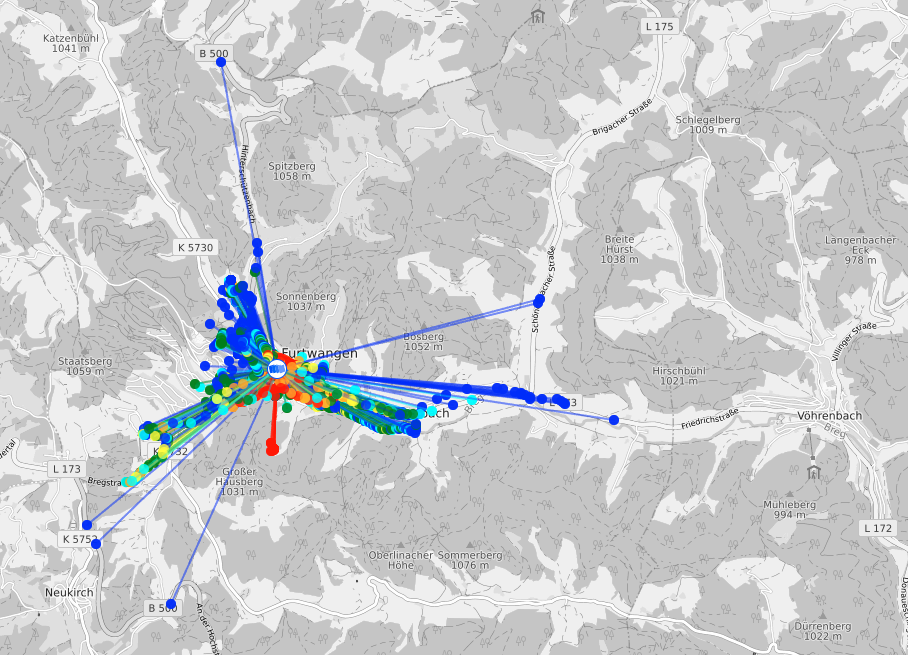
\includegraphics[width=1\textwidth]{pictures/ttn-mapper/gateway-ranges/c_building_gw_range.png}
    \caption[Screenshot of a \acl{TTNM} map showing some data points taken from the \acl{LRWGW} deployed on top of the C building]{
        Screenshot of a \ac{TTNM} map showing some data points taken from the \acl{LRWGW} deployed on top of the C building.
        The slightly smaller range compared to \Cref{pic:ghb_mikrotik_gw_range} is evident.
        The maximum range, however, is still \SI{4.3}{\kilo\meter} which is the rightmost blue point in the direction of Vöhrenbach~\cite{ttn_mapper_ttn_2023}.
    }\label{pic:c_building_gw_range}
\end{figure}

\Cref{pic:c_building_gw_range} shows the range of the \ac{HFU} C building \acl{LRWGW}.
Clearly visible is the slightly smaller range compared to \Cref{pic:ghb_mikrotik_gw_range}.
The maximum range recorded for this \acl{LRWGW} is \SI{4.3}{\kilo\meter}, which is the rightmost blue point in the direction of Vöhrenbach again.

Installing the \acl{LRWGW} on the roof of the \ac{HFU} C building was rather easy since accessing the roof is not difficult.
The cable of the antenna had to be pulled through a small conduit in the outer wall.
Afterward, it could be connected to the \acl{LRWGW} located inside a small crawl space.

Getting the network backhaul up and running wasn't as straightforward, though.
There were no spare Ethernet ports available in the crawl space.
However, there was a spare fiber optic cable run that was not in use at the moment.
Using two media converters, the fiber optic cable was converted to Ethernet and connected to the \ac{HFU} network one story below the roof.

\subsection{\acl{ASH}}

Installing the \acl{LRWGW} on the roof of the \ac{ASH} building was an arduous task, but it was worth it.
The roof is difficult to access, and the \acl{LRWGW} had to be installed on top of an antenna mast.

Getting a backhaul connection was rather easy, since a \ac{PoE} switch was available in the server room just beneath the roof.

The range, as shown in \Cref{pic:ash_gw_range}, is very good and covers almost the entire Furtwangen area.
It is similar to the coverage of the \ac{GHB} building, since the \ac{ASH} building is also a multi-story building on a hill.

\begin{figure}[htbp]
    \centering
    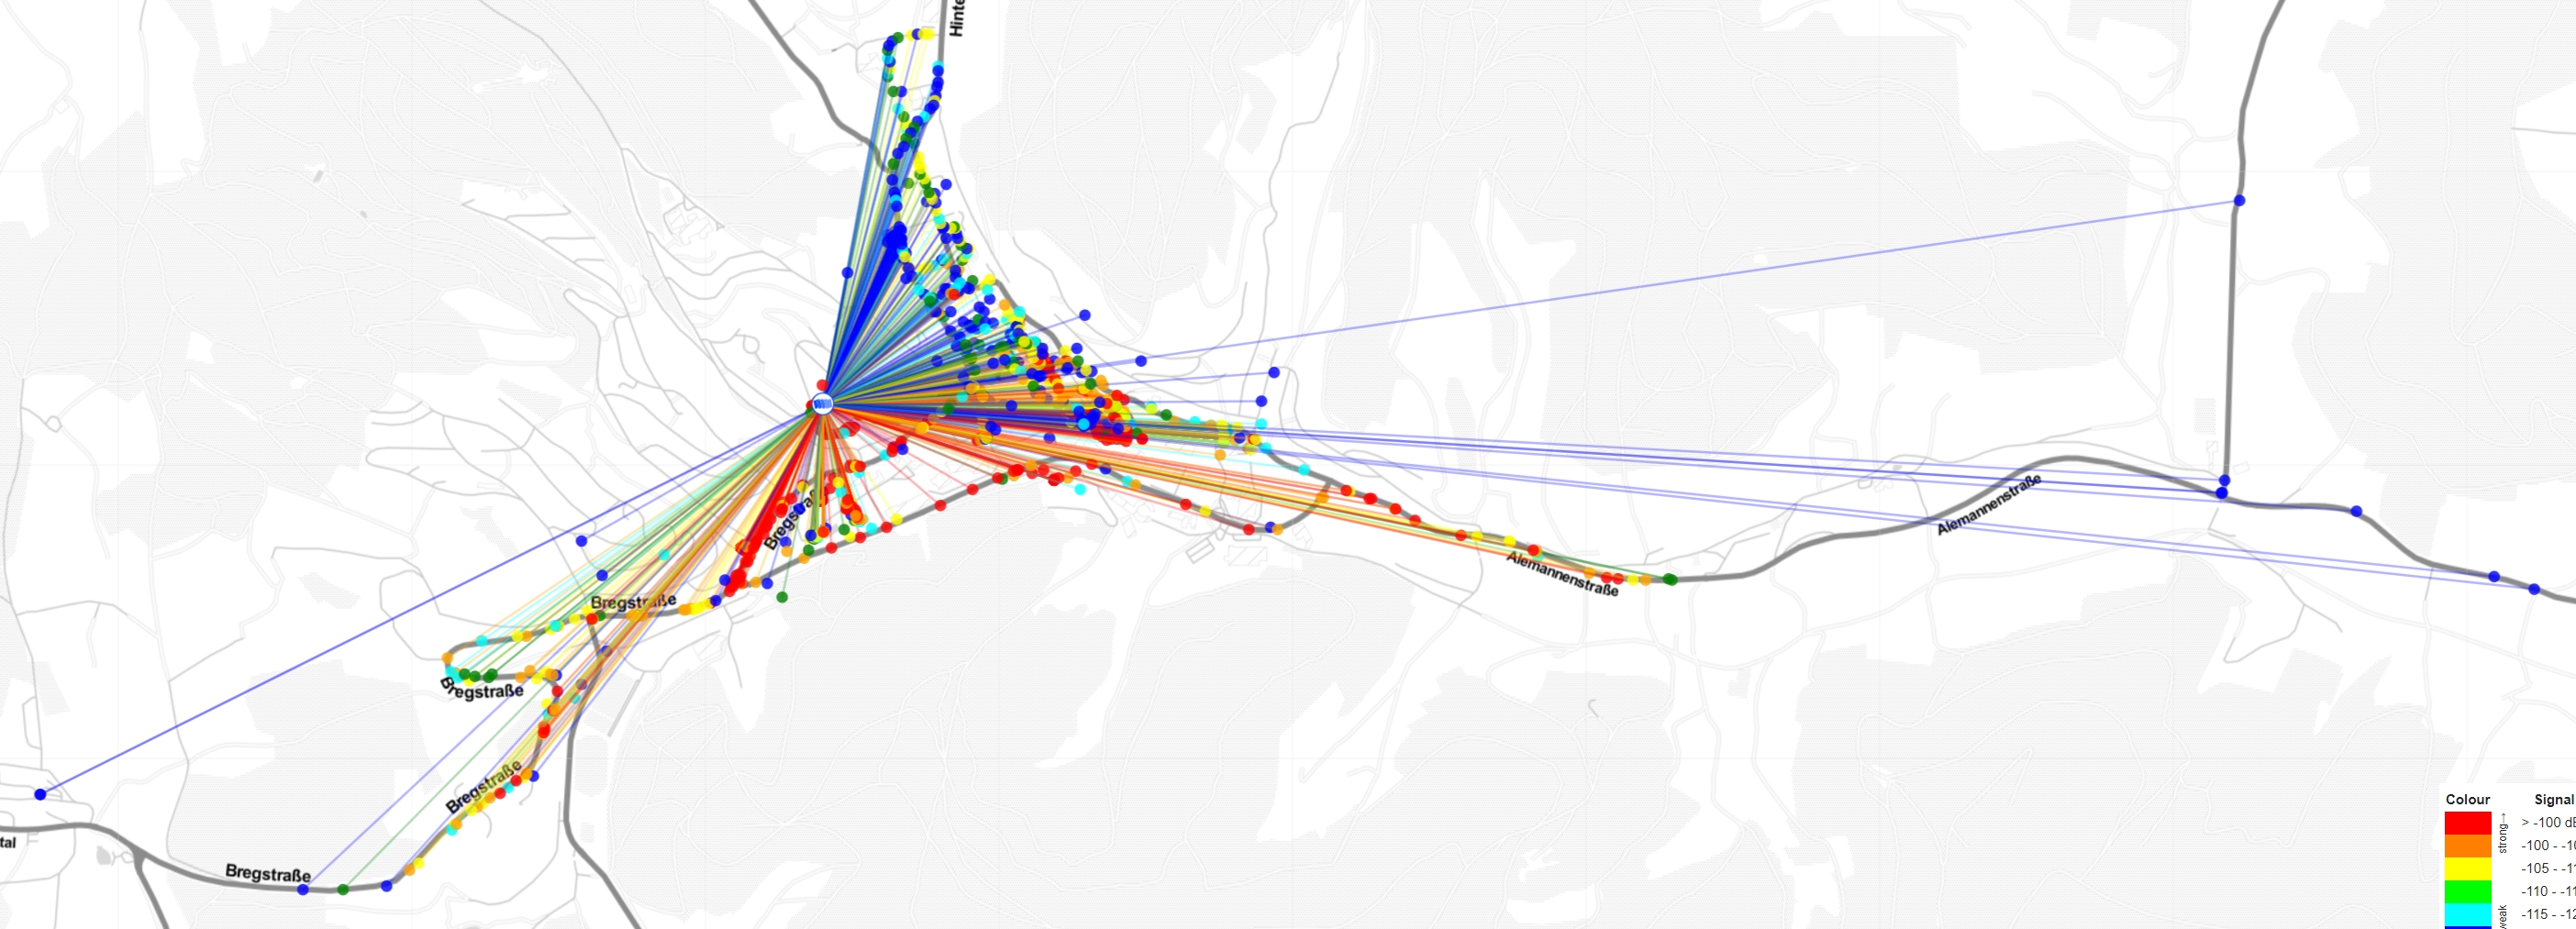
\includegraphics[width=1\textwidth]{pictures/ttn-mapper/gateway-ranges/ash_gw_range.jpg}
    \caption[Screenshot of a \acl{TTNM} map showing some data points taken from the \acl{LRWGW} deployed on the roof of the \acl{ASH} building]{
        Screenshot of a \ac{TTNM} map showing some data points taken from the \acl{LRWGW} deployed on the roof of the \ac{ASH} building.
        It has a good range into most parts of the Furtwangen area~\cite{ttn_mapper_ttn_2023}.
    }\label{pic:ash_gw_range}
\end{figure}

The longest range recorded from the \ac{ASH} building thus far is around \SI{4.8}{\kilo\meter} which is the blue point on the right of \Cref{pic:ash_gw_range}.

\subsection{DL0FIS amateur radio club station}

While the location of the \ac{LoRaWAN} on top of a hill between Furtwangen and Gütenbach should have made for very good coverage, the reality looks different.

\begin{figure}[htbp]
    \centering
    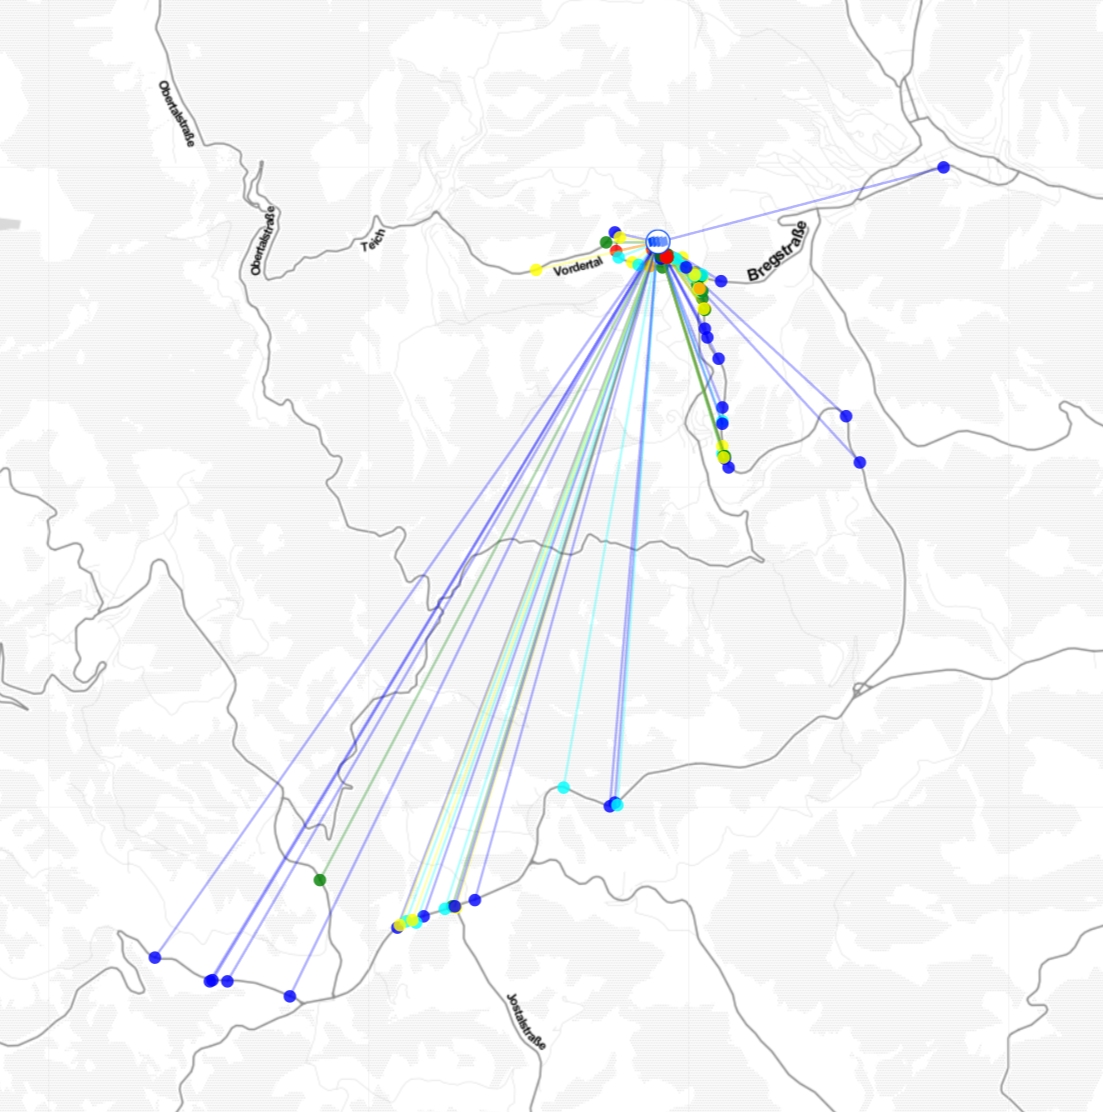
\includegraphics[width=.8\textwidth]{pictures/ttn-mapper/gateway-ranges/dl0fis_gw_range.jpg}
    \caption[Screenshot of a \acl{TTNM} map showing data points taken from the \acl{LRWGW} deployed on the roof of the DL0FIS clubhouse]{
        Screenshot of a \ac{TTNM} map showing data points taken from the \acl{LRWGW} deployed on the roof of the DL0FIS clubhouse.
        While the range is not consistent in every direction due to the hills and mountains in the area, the longest range of around \SI{8.8}{\kilo\meter} is still very good.
        Coverage of Furtwangen is almost nonexistent due to the hills in the way~\cite{ttn_mapper_ttn_2023}.
    }\label{pic:dl0fis_gw_range}
\end{figure}

\Cref{pic:dl0fis_gw_range} shows the coverage of the \acl{LRWGW} deployed on the roof of the DL0FIS clubhouse.
The longest range measured was one data point in the south with a distance of \SI{8.8}{\kilo\meter}.

\begin{figure}[htbp]
    \centering
    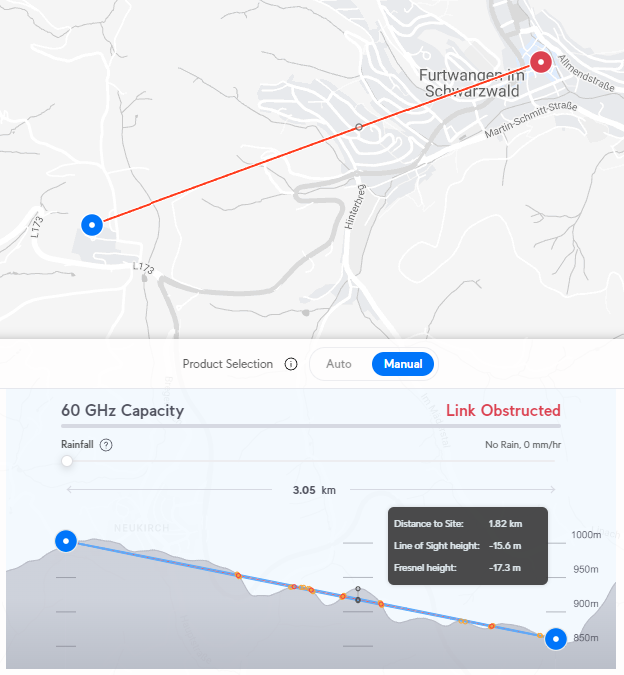
\includegraphics[width=.6\textwidth]{pictures/hardware/gateway-deployment/line-of-sight-dl0fis.png}
    \caption[\acl{LoS} between the DL0FIS clubhouse and the Furtwangen city center]{
        Screenshot of the Ubiquiti UISP Design Center tool.
        It displays the \ac{LoS} between two points with customizable antenna elevation and can show any terrain elevation between them.
        The multiple hills blocking the signal from the DL0FIS clubhouse to the Furtwangen city center are visible~\cite{ubiquiti_inc_uisp_2023}.
    }\label{pic:dl0fis_gw_los}
\end{figure}
    
The \acl{LRWGW}, up until now, was not of much use in the scope of this thesis though, since the hill between the Neueck clubhouse and Furtwangen blocks most of the signal.
\Cref{pic:dl0fis_gw_los} shows those obstructions.

Getting a backhaul connection to the \acl{LRWGW} was easy since the clubhouse is equipped with a stable, wired internet connection.
The gateway could thus be connected using Ethernet.

\subsection{\acl{HFU} O building}\label{subsec:conclusion-hfu-o-building}

Another possible location that was not mentioned in \Cref{sec:gateway-locations} was the \ac{HFU} O building.
Located in the northern part of Furtwangen, it is a multi-story building that used to be a hospital.
Since the \ac{HFU} is only a tenant there, permission was needed from the building owner to install the gateway.
Fortunately, the owner, Mr.\ Odin Jäger, was very cooperative and allowed the gateway to be installed.

Unfortunately, it was not as easy to get a network connectivity and power on the roof as it was in the other buildings, so no gateway has been installed there yet.
This may be done in the future if a way can be found to get a network and power to the roof.

\subsection{Factory building of the E. Wehrle GmbH company}\label{subsec:factory-building-of-the-e-wehrle-company}

During the initial weeks of collecting data with \ac{GPS} trackers in Furtwangen, a gateway without location information appeared in the \ac{TTN} packet metadata.
Upon further investigation, it was discovered that the gateway was situated on the factory building roof of E. Wehrle GmbH, a company located in the eastern region of Furtwangen.
After contacting the company, Tom Lehmann, an external consultant for the company working at Netzint GmbH, was very cooperative and entered its location into the \ac{TTN} console.
This allowed the gateway to be displayed on the \ac{TTNM} map and for its data to also be considered in the \ac{TTNL} calculations.

The E. Wehrle GmbH company is a manufacturer of (among other products) smart metering sensors.
Alongside other protocols, they also use \ac{LoRaWAN} for some of their products~\cite{e_wehrle_gmbh_wecount-s_nodate}.

\section{Collected data in Furtwangen on \acl{TTNM}}\label{sec:collected-data-in-furtwangen-on-ttnm}

\subsection{\acl{TTNM} heatmap view after additional data collection}\label{sec:ttm_heatmap_after}

During this thesis, additional data was collected using the \ac{LoRaWAN} \ac{GPS} trackers mentioned in \Cref{subsec:used-lora-devices}.
This lead to a denser data coverage of \acl{TTNM} in the Furtwangen area.

\begin{figure}[htbp]
    \centering
    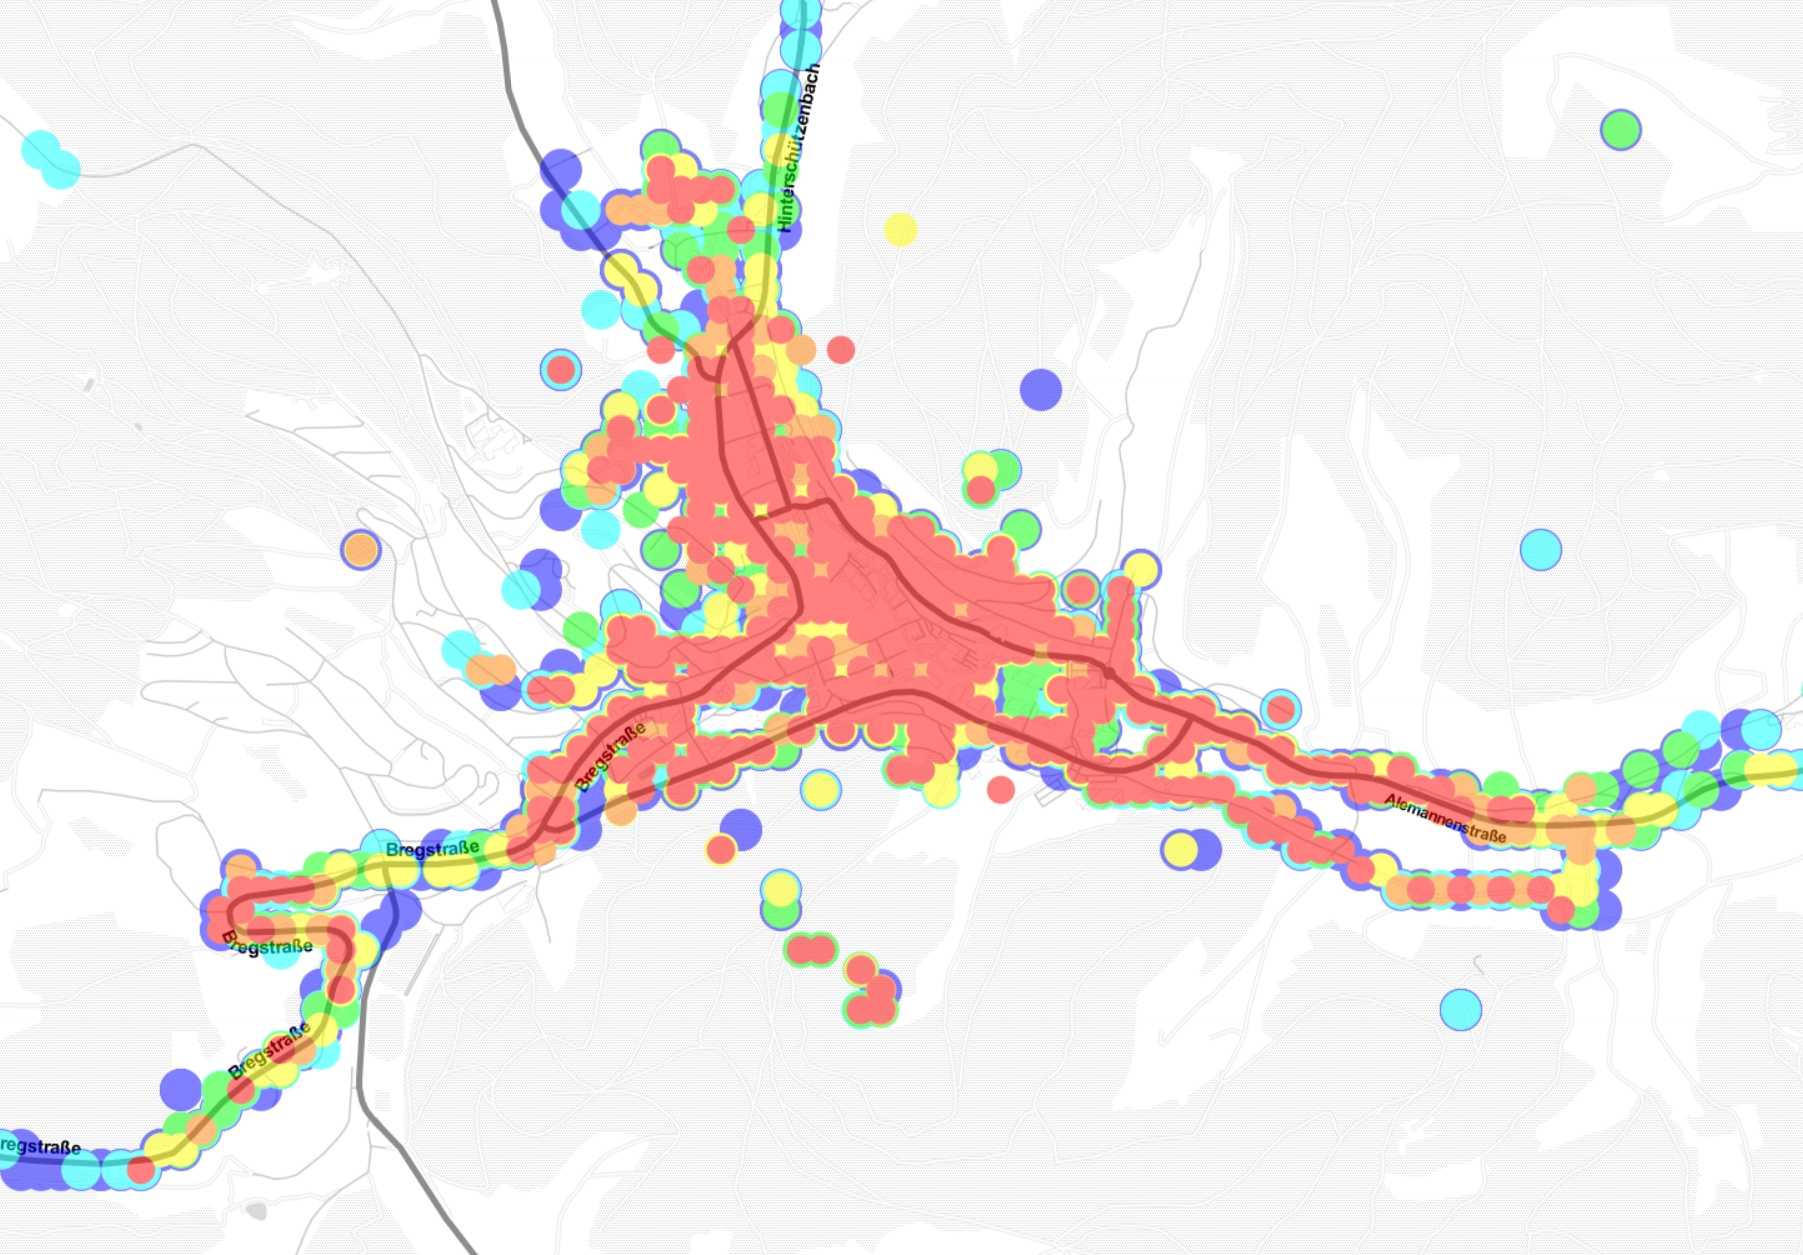
\includegraphics[width=0.7\textwidth]{pictures/ttn-mapper/ttnm_heatmap_after_data_collection.jpg}
    \caption[Screenshot of the \acl{TTNM} heatmap view after data collection during this thesis, from the 21st of June 2023]{
        Screenshot of the \ac{TTNM} heatmap view after data collection during this thesis, from the 21st of June 2023.
        Compared to \Cref{pic:ttnm-before-data-collection}, the coverage has improved significantly.
        Several \aclp{LRWGW} were deployed as well as the additional data collection performed with \ac{LoRaWAN} \ac{GPS} trackers~\cite{ttn_mapper_ttn_2023}.
    }\label{pic:ttnm-heatmap-after-data-collection}
\end{figure}

\Cref{pic:ttnm-heatmap-after-data-collection} shows a view of the \ac{TTNM} heatmap after the additional data collection that was done during this thesis.
The much redder color of the map is visible, meaning that the signal strength measured in these areas is stronger than before, as visible in \Cref{pic:ttn-mapper-heatmap-with-gateways}.

While there are still some blank spots on the map, these are mostly due to the fact that these areas were not visited by \ac{GPS} trackers during the data collection in this thesis.

\section{Comparison of Geolocation Methods}

This section will compare the different geolocation methods that were used in this thesis.

\subsection{Methods using the multilateration approach}\label{subsec:conclusion-multilateration}

\subsubsection{\acl{RSSI}}

\Cref{lst:sql-calculate-correlation-coefficient} shows a \ac{SQL} query that was used to calculate the correlation coefficient between \ac{RSS} values and their associated distances for a single gateway.
Its purpose is to show how much the \ac{RSS} values correlate with the distance between the \acl{ED} and the \ac{GW}.

\begin{lstlisting}[
    language=SQL,
    float,
    caption={[\acl{SQL} query used to calculate the correlation coefficient between \acl{RSS} values and associated distances]
        \ac{SQL} query used to calculate the correlation coefficient between \ac{RSS} values and associated distances for a single gateway.
        This query was also generated by Bing AI and adjusted to fit the the application's needs.
        The \lstinline|CORR| function was used to calculate the correlation coefficient over the gateway's data points.
    },
    label={lst:sql-calculate-correlation-coefficient}
]
WITH gateway_data AS (
    SELECT
        gateway.latitude AS gateway_latitude,
        gateway.longitude AS gateway_longitude,
        deviceGPSDatapoint.latitude AS datapoint_latitude,
        deviceGPSDatapoint.longitude AS datapoint_longitude,
        ttnMapperDatapoint.rssi AS rssi
    FROM
        "Gateway" gateway
        JOIN "TtnMapperDatapoint" ttnMapperDatapoint ON gateway."gatewayId" = ttnMapperDatapoint."gatewayId"
        JOIN "DeviceGPSDatapoint" deviceGPSDatapoint ON ttnMapperDatapoint."deviceGPSDatapointId" = deviceGPSDatapoint.id
    WHERE
        gateway."gatewayId" = 'hfu-lr8-001'
),
distance_data AS (
    SELECT
        *,
        ST_DistanceSphere(
            ST_MakePoint(gateway_longitude, gateway_latitude),
            ST_MakePoint(datapoint_longitude, datapoint_latitude)
        ) AS distance
    FROM
        gateway_data
),
stats_data AS (
    SELECT
        CORR(distance, rssi) AS correlation_coefficient,
		COUNT(*) AS datapoint_count
    FROM
        distance_data
)
SELECT * FROM stats_data;
\end{lstlisting}

The result for a data set of about \num{10000} collected ttnMapperDatapoints from the \ac{GHB} MikroTik gateway is roughly equal to \num{-0.261}, indicating a medium to weak negative correlation between the \ac{RSS} values and the distance to the gateway~\cite{taylor_interpretation_1990}.
Other gateways show similar results.

This means that, in general real-world scenarios, \ac{RSS} values alone are not a reliable indicator for determining distances.
Still, this section will provide an overview over the techniques used during this thesis to estimate the position of a \acl{ED} based on \ac{RSS} values in two different ways.

\paragraph{Accuracy of multilateration based on \aclp{RSS} with a fixed \acl{RSS} to range function}\label{subsubsec:conclusion-rssi-fixed-scale}

As shown in \Cref{sec:fixed-rssi-to-range-scale-impl}, a fixed \ac{RSS} to range mapping was implemented in the frontend first.
In general, the accuracy of using such a fixed \ac{RSSI} to range mapping was poor.

\begin{figure}[htbp]
    \centering
    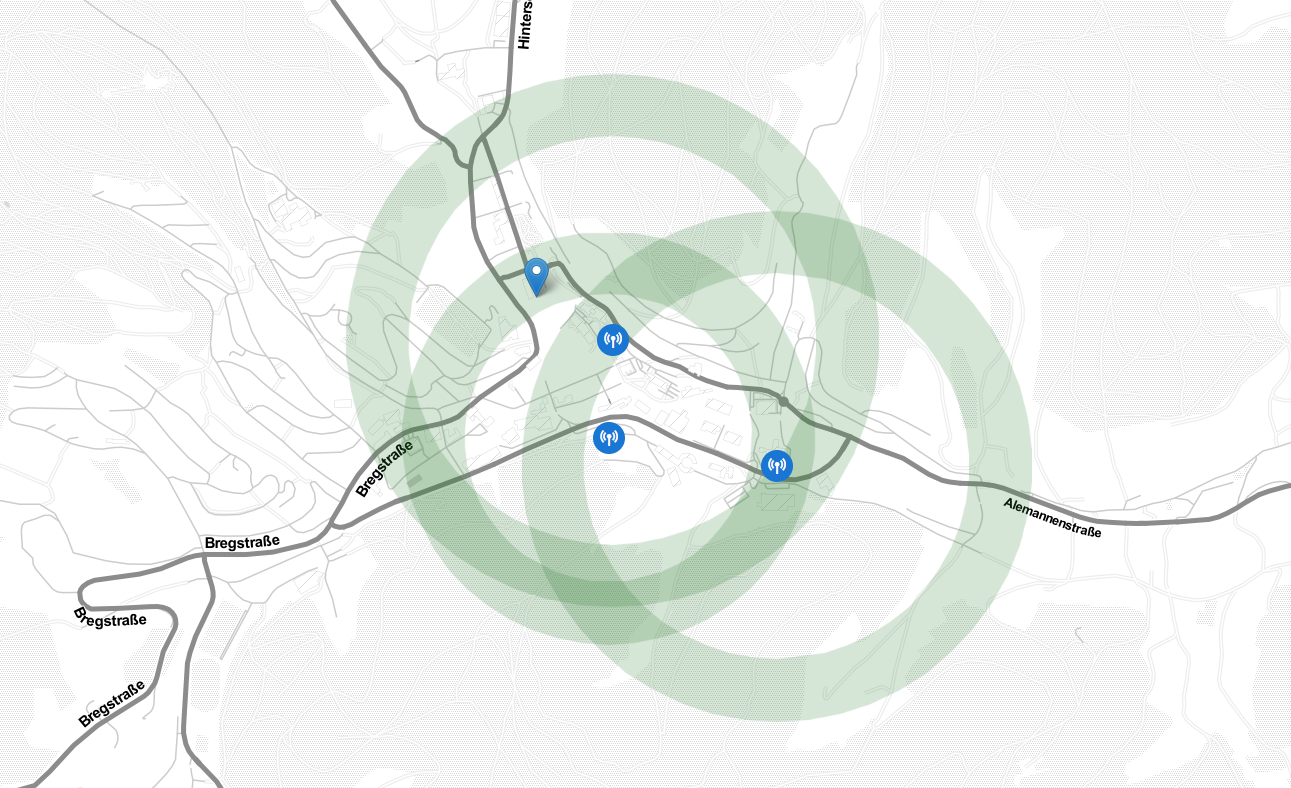
\includegraphics[width=0.8\textwidth]{pictures/ttn-locator/frontend/multilateration/rssi_range_multilateration_bad_example.png}
    \caption[Screenshot of the \acl{TTNL} frontend showing an example of a multilateration using a fixed \acl{RSSI} to range mapping]{
        Screenshot of the \ac{TTNL} frontend showing an example of a multilateration with three \aclp{LRWGW} using a fixed \ac{RSSI} to range mapping.
        It can be seen that the estimated position, where the three green annuli intersect, is quite far away from the actual position (blue pin) of the \acl{ED}.
        The width of the annuli is an arbitrary value of \SI{100}{\meter} in this case.
        The value can be changed in the frontend to test various error margins.
        The annuli are drawn using Leaflet's ability to render GeoJSON.\@
    }\label{pic:bad-rssi-to-range-multilateration-example}
\end{figure}

\Cref{pic:bad-rssi-to-range-multilateration-example} shows an example of a multilateration with a fixed \ac{RSSI} to range mapping where the result is not at all accurate.

\paragraph{Accuracy of multilateration based on \aclp{RSS} with linear regression per gateway}\label{subsubsec:conclusion-rssi-linear-regression}

As mentioned in \Cref{subsubsec:per-gateway-rssi-to-range-scale}, another idea was to use linear regression to create a \ac{RSS} to range function to map \ac{RSS} values to ranges for each gateway.
This approach considers gateway-specific parameters such as position and gateway antenna gain.
However, it cannot consider \ac{MPP} effects as well as \acl{ED} antenna gain.

\begin{figure}[htbp]
    \centering
    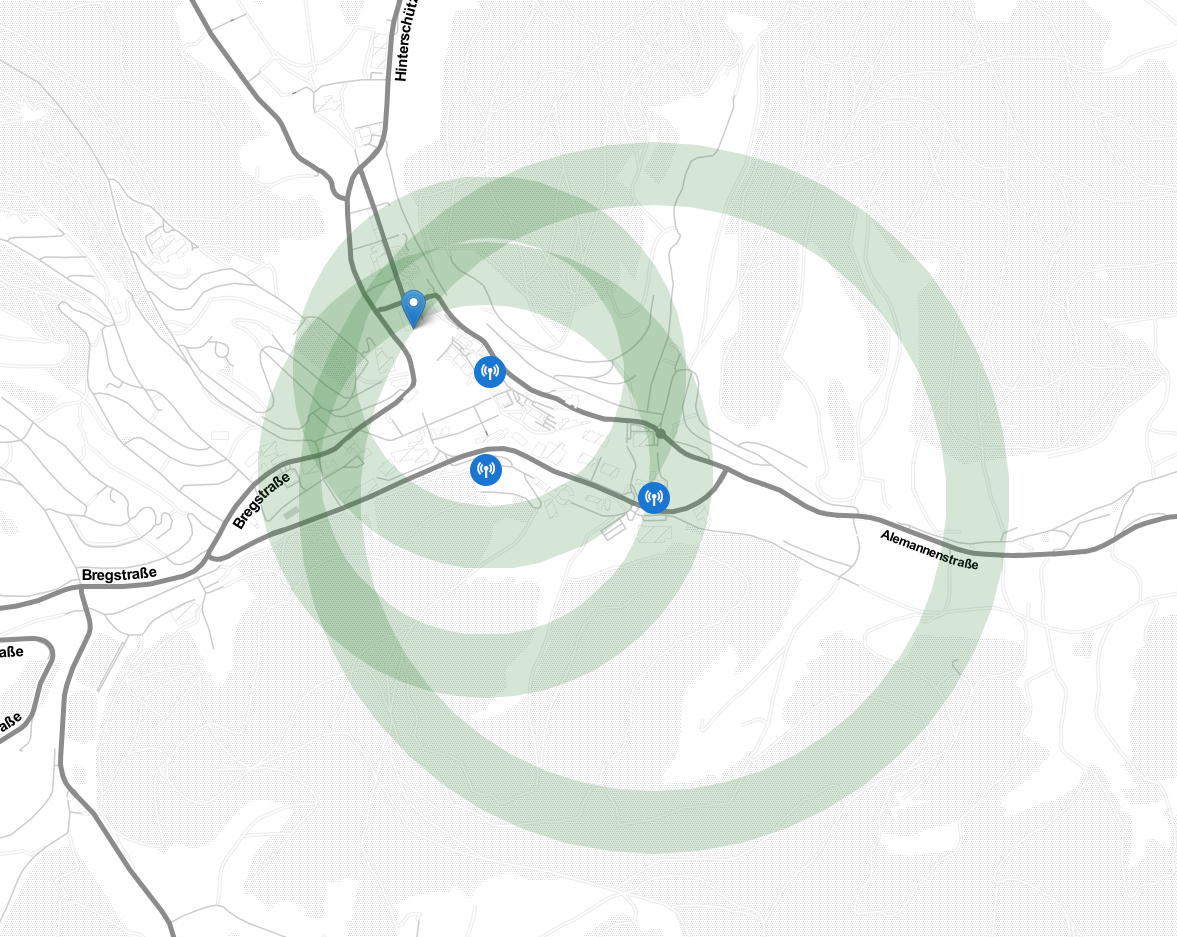
\includegraphics[width=0.8\textwidth]{pictures/ttn-locator/frontend/multilateration/rssi_range_multilateration_regression_example.png}
    \caption[Screenshot of the \acl{TTNL} frontend showing an example of a multilateration using a linear regression based \acl{RSSI} to range mapping]{
        Screenshot of the \ac{TTNL} frontend showing an example of a multilateration with three \aclp{LRWGW} using a linear regression based \ac{RSSI} to range mapping per gateway.
        It uses the same base data point as seen in \Cref{pic:bad-rssi-to-range-multilateration-example}.
        The estimated position, where the three green annuli intersect, is more accurate compared to the fixed range mapping.
        The width of the annuli is, again, an arbitrary value of \SI{100}{\meter}.
    }\label{pic:rssi-to-range-multilateration-example-with-linear-regression}
\end{figure}

\Cref{pic:rssi-to-range-multilateration-example-with-linear-regression} shows an example of the same parameters as in \Cref{pic:bad-rssi-to-range-multilateration-example} but with a linear regression model that determines a mapping of \ac{RSS} values to ranges for each gateway.
The example shows that the resulting position estimation where the three annuli intersect is better than in \Cref{pic:bad-rssi-to-range-multilateration-example}.
However, since the linear regression model cannot account for \ac{MPP} effects either, the results still typically deviate from the actual position by a few hundred meters.

\paragraph{Conclusion: \acl{RSS} approaches}

As was explained in \Cref{sec:multipath-propagation}, \acl{MPP} effects can cause the \ac{RSS} values to fluctuate heavily.
In addition, as explained in \Cref{sec:rssi}, different antennas on \aclp{LRWGW} and \aclp{LRWED} can cause different \ac{RSS} values to be measured for the same distance due to different antenna gains.

This makes multilateration with \ac{RSS} values as the only input data unreliable for precise geolocation.
Even when using a linear regression model to generate a mapping of \ac{RSS} values to ranges for each gateway, the results were often only accurate to several hundred meters.

\subsubsection{\acl{ToA}}\label{subsec:conclusion-toa-tdoa}

\Cref{subsec:toa-based-multilateration-implementation} mentioned the fact that using timestamps from \aclp{LRWGW} to determine the range to the \acl{ED} are too inaccurate to be used for \ac{ToA}-based geolocation.

In addition to the fact that timestamps arrive at \ac{TTN} with unrealistic offsets due to missing time synchronization as seen in \Cref{fig:toa-bad-data-example}, another factor has to be considered.
\ac{TTN} captures timestamps for packets arriving at \aclp{LRWGW} in the following format: \lstinline|2000-01-01T12:00:00.123456Z|.
These timestamps can be found in the \lstinline|uplink_message.rx_metadata[*].time| field of the \ac{JSON} payload that can be viewed in the \ac{TTN} console for each packet that arrives from a certain \acl{ED}~\cite{the_things_industries_bv_data_2023}.
It uses the \ac{ISO} 8601 \ac{UTC} standard for timestamps~\cite{newman_date_2002}.
The six decimal places after the seconds mean that the timestamp is accurate to \SI{1}{\micro\second}.
\Cref{eq:toa-accuracy-ttn-microseconds} shows that when using microseconds to calculate the distance to a \acl{LRWGW} based on the speed of light, a maximum accuracy of \SI{300}{\meter} can be achieved.

\begin{equation}\label{eq:toa-accuracy-ttn-microseconds}
    \text{ToA\,accuracy}_{\si{\micro\second}} = \frac{299792458 \frac{\si{\meter}}{\si{\second}}}{10^6} \approx 300 \si{\meter}
\end{equation}

\Cref{eq:toa-accuracy-ttn-nanoseconds} shows that using nanoseconds, a much better accuracy of \SI{0.3}{\meter} could be achieved.

\begin{equation}\label{eq:toa-accuracy-ttn-nanoseconds}
    \text{ToA\,accuracy}_{\si{\nano\second}} = \frac{299792458 \frac{\si{\meter}}{\si{\second}}}{10^9} \approx 0.3 \si{\meter}
\end{equation}

Solving these problems on the scope of the entire \ac{TTN} network is not feasible because it would require synchronizing the clocks of all \aclp{LRWGW} in the network with \ac{GPS} receivers or in another way.
However, if one were to deploy a \ac{LoRaWAN} network in a smaller area where control over every \acl{LRWGW} is realistic, this would be a possible solution.
If every gateway in the network were accurately time-synchronized and \si{\nano\second}-level timestamps could be used, \ac{ToA} would be a viable option for geolocation.

\subsection{Fingerprinting}\label{subsec:conclusion-fingerprinting}

This section evaluates the fingerprinting approach as described in \Cref{sec:fingerprinting-implementation}.

\subsubsection{\acl{RSS} only}

\Cref{fig:fingerprinting-map-example-only-center} already showed an example where the center of matching filtered data points was taken as the estimated position, along with an arbitrary radius to show the associated uncertainty.

\begin{figure}[htbp]
    \centering
    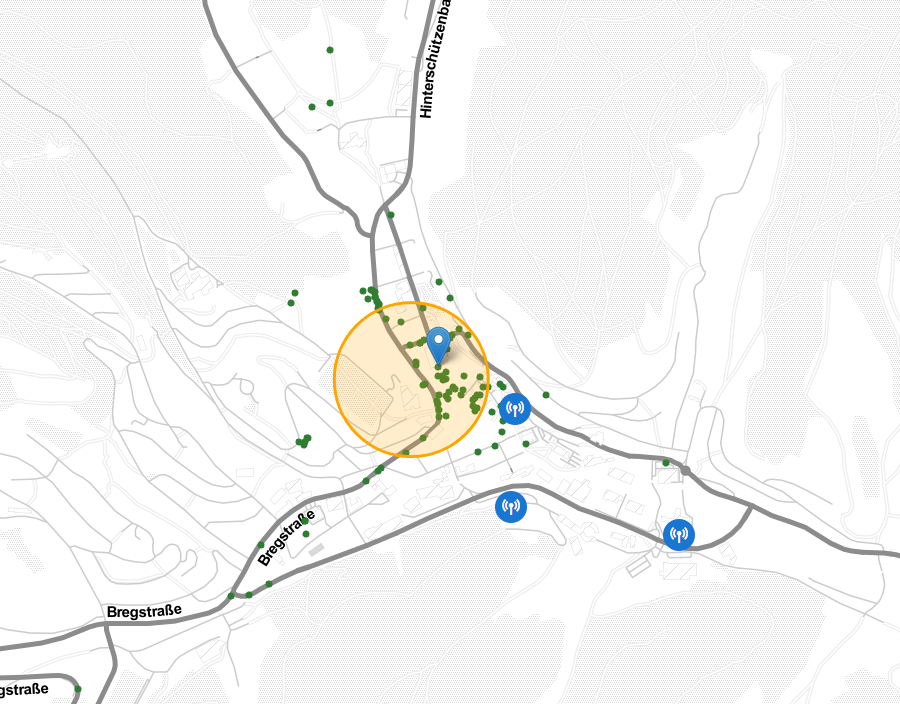
\includegraphics[width=0.6\textwidth]{pictures/ttn-locator/frontend/fingerprinting/rssi_similarity_map_example_dynamic_radius.png}
    \caption[Example for a fingerprinting result map generated by \acl{TTNL} with \acl{RSS} values only]{
        Screenshot of the \ac{TTNL} frontend showing an example for a fingerprinting result map generated by \ac{TTNL}.
        The blue pin shows the actual position of the \acl{ED}.
        The yellow circle shows the estimated position that \ac{TTNL} calculated out of the center of the matching data points.
        The radius is determined by having half of the matched points fit inside it.
    }\label{fig:fingerprinting-map-example-dynamic-radius}
\end{figure}

On the other hand, \Cref{fig:fingerprinting-map-example-dynamic-radius} shows an approach where the error radius is not arbitrary, but is calculated based on fitting half the matched points inside the circle.
This usually results in a larger error radius (low precision), but a higher rate of actually containing the actual position (high accuracy).

\subsubsection{Adding \acl{SNR}}


As mentioned in \Cref{sec:adding-snr-to-fingerprinting}, \ac{SNR} values were also used in the fingerprinting approach in addition to \ac{RSSI}.
Even though \ac{SNR} values are also affected by \ac{MPP} effects, this improved the accuracy of the results in some cases.
However, since \ac{SNR} values also depend on the \ac{SF} used, both should be used in conjunction if the fingerprint \ac{DB} contains data with varying \acp{SF}.

\begin{figure}[htbp]
    \centering
    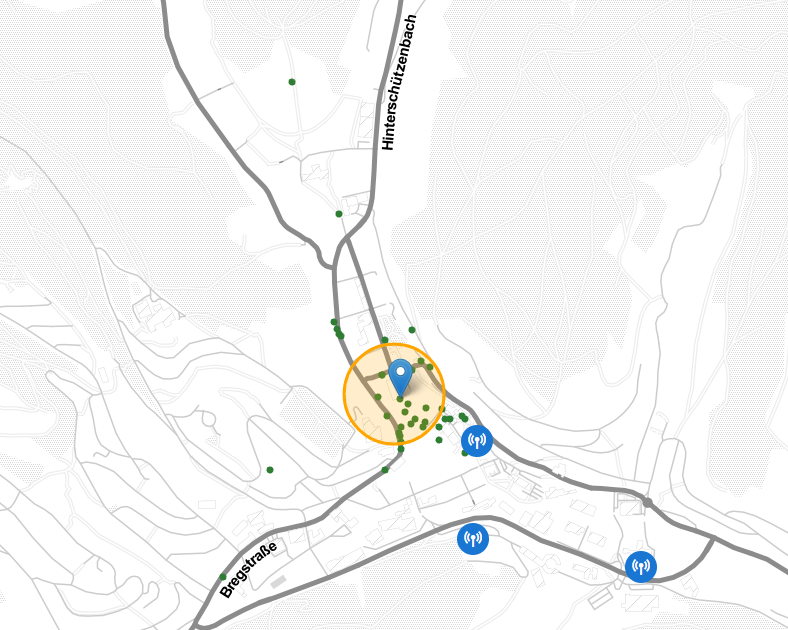
\includegraphics[width=0.6\textwidth]{pictures/ttn-locator/frontend/fingerprinting/fingerprinting_map_example_with_snr.png}
    \caption[Example for a fingerprinting result map generated by \acl{TTNL} with \acl{RSS} and \acl{SNR} values]{
        Screenshot of the \ac{TTNL} frontend showing an example for a fingerprinting result map generated by \ac{TTNL}.
        In addition to the example provided in \Cref{fig:fingerprinting-map-example-dynamic-radius}, this example also includes \ac{SNR} values.
    }\label{fig:fingerprinting-map-example-with-snr}
\end{figure}

\Cref{fig:fingerprinting-map-example-with-snr} shows an example of a position estimate where \ac{SNR} values were used in addition to \ac{RSS} values.

A disadvantage of this approach would be that it would require more data to be stored, since the number of possible variables per captured gateway would increase from 1 (\ac{RSSI}) to 2 or even 3 (\ac{RSSI}, \ac{SF}, \ac{SNR}).
Nevertheless, data collection is not a problem, since \ac{TTN} already captures all of those values with each received data frame.

\subsubsection{Adding \acl{SF}}

As mentioned in \Cref{sec:sf-snr-correlation}, the \ac{SF} used by the \acl{ED} has an influence on the \ac{SNR} values at which a signal can still be detected.
This means that the \ac{SF} value also plays a role in a more accurate location estimation of the \acl{ED}.

The \ac{TTNL} frontend includes a checkbox that enables the addition of \ac{SF} values to the fingerprinting filter.
This prevents data points from \acp{SF} different from the one used by the \acl{ED} from being included in the filter.
That way, the \ac{SNR} values of the remaining data points are applicable to the actual \ac{SNR} values of the \acl{ED}.

\begin{figure}[htbp]
    \centering
    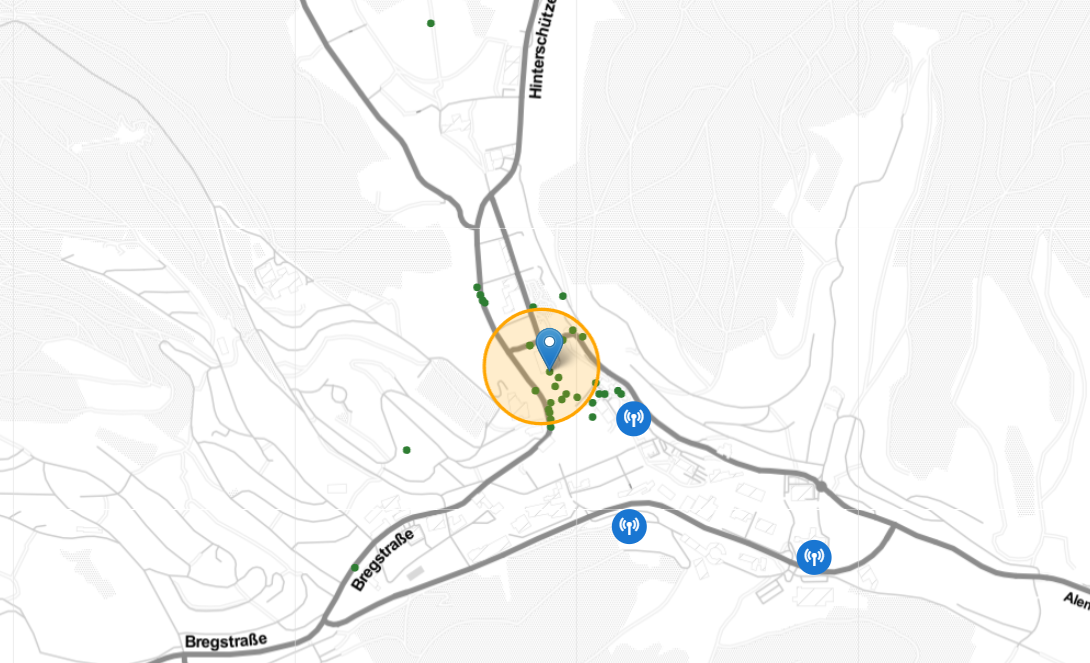
\includegraphics[width=0.7\textwidth]{pictures/ttn-locator/frontend/fingerprinting/fingerprinting_map_example_with_snr_sf.png}
    \caption[Example for a fingerprinting result map generated by \acl{TTNL} with \acl{RSS}, \acl{SF} and \acl{SNR} values]{
        Screenshot of the \ac{TTNL} frontend showing an example for a fingerprinting result map generated by \ac{TTNL}.
        In addition to the example provided in \Cref{fig:fingerprinting-map-example-with-snr}, this example also filter according to the data point's \ac{SF} value.
    }\label{fig:fingerprinting-map-example-with-snr-and-sf}
\end{figure}

\Cref{fig:fingerprinting-map-example-with-snr-and-sf} shows an example with \ac{SF} filtering turned on.
The result is dependent on the amount of training data that was collected for the area, but for most cases, also filtering by \ac{SF} further improves the accuracy of the results.
This is because it removes results with a \ac{SF} different from the one used by the \acl{ED}, which could otherwise have \ac{SNR} values different from the actual \acl{ED} packets.
As most \aclp{LRWED} used in this thesis were using \ac{SF}7, the example given in \Cref{fig:fingerprinting-map-example-with-snr-and-sf} doesn't show much improvement of accuracy over \Cref{fig:fingerprinting-map-example-with-snr}.
However, if a larger dataset with a greater variation of \ac{SF} values were used, the improvement would be more visible.

\subsubsection{Conclusion}

In comparison to the multilateration approach, the fingerprinting approach is not easily scalable.
It requires considerable manual work to create a fingerprint \ac{DB} for a certain area.
This makes it only feasible for smaller, contained areas and rather unusable for larger-scale geolocation such as in a whole city or state.
While the accuracy of the fingerprinting approach improves with more training data, collecting a large quantity of training data for a large area may not be feasible.

However, the results of the fingerprinting approach are, in general more accurate than the results of the multilateration approach.
This is because it can take into account the \ac{SF} and \ac{SNR} values of the \acl{ED}, which are not available in the multilateration approach.
In addition, performance inside buildings is also better than with the multilateration approach, since the fingerprinting approach does not assume \ac{LoS} between the \acl{LRWED} and the \aclp{LRWGW}.
Thus, it can also take into account the \ac{MPP} effects such as attenuation that occur inside buildings or behind walls.

In the example pictures given in \Cref{fig:fingerprinting-map-example-dynamic-radius}, \Cref{fig:fingerprinting-map-example-with-snr} and \Cref{fig:fingerprinting-map-example-with-snr-and-sf}, the error radii improved from around \SI{250}{\meter} with only \ac{RSS} values to \SI{159}{\meter} with \ac{SNR} values and around \SI{164}{\meter} with \ac{SNR} and \ac{SF} values.
The worse performance with both \ac{SF} and \ac{SNR} values can be explained due to the fact that the amount of training data for the area did not include many \aclp{SF} other than \acs{SF}7.

\section{Comparison of findings with existing work}

Several of the approaches found in \Cref{sec:related-work} have better success in locating endpoints than the work in this thesis.
This could be due to the fact that these approaches use more tightly controlled environments, such as having \ac{LoS} between the \acl{LRWED} and the \aclp{LRWGW}.
Additionally, most of these approaches use smaller testing areas, such as a single building or a small campus, as opposed to the entire city of Furtwangen.
However, the work presented in this thesis was successful in achieving rough geolocation.

The hardware deployments in this thesis were less focused on getting good geolocation results and more focused on getting a large amount of data from a wide variety of \aclp{ED} and \aclp{GW}.
This variety is also the case in real-world \ac{IoT} deployments.
As far as \ac{LoRaWAN} coverage in the Furtwangen is concerned, this can be considered a success.
As was shown in \Cref{sec:gateway-locations-conclusions}, \ac{LoRaWAN} coverage in Furtwangen on \ac{TTNM} now looks a lot more complete than it did before the work during this thesis (\Cref{pic:ttnm-before-data-collection}).

\section{Outlook}

This section will provide an outlook on possible future work that could be done in relation to this thesis.

\subsection{Improving the \acl{TTNL} software}

This section will mention some ideas on how to improve the \ac{TTNL} software.

\subsubsection{Automatically detecting \aclp{LRWGW} that have been relocated}

Although uncommon, it is conceivable for a \acl{LRWGW} to be relocated after it has been registered in the \ac{TTN} \ac{LNS}.
Thus, since the \ac{TTNL} software currently updates the gateway locations after each \ac{TTNM} data collection run, it is possible that outdated data could alter location estimations.

\begin{figure}[htbp]
    \centering
    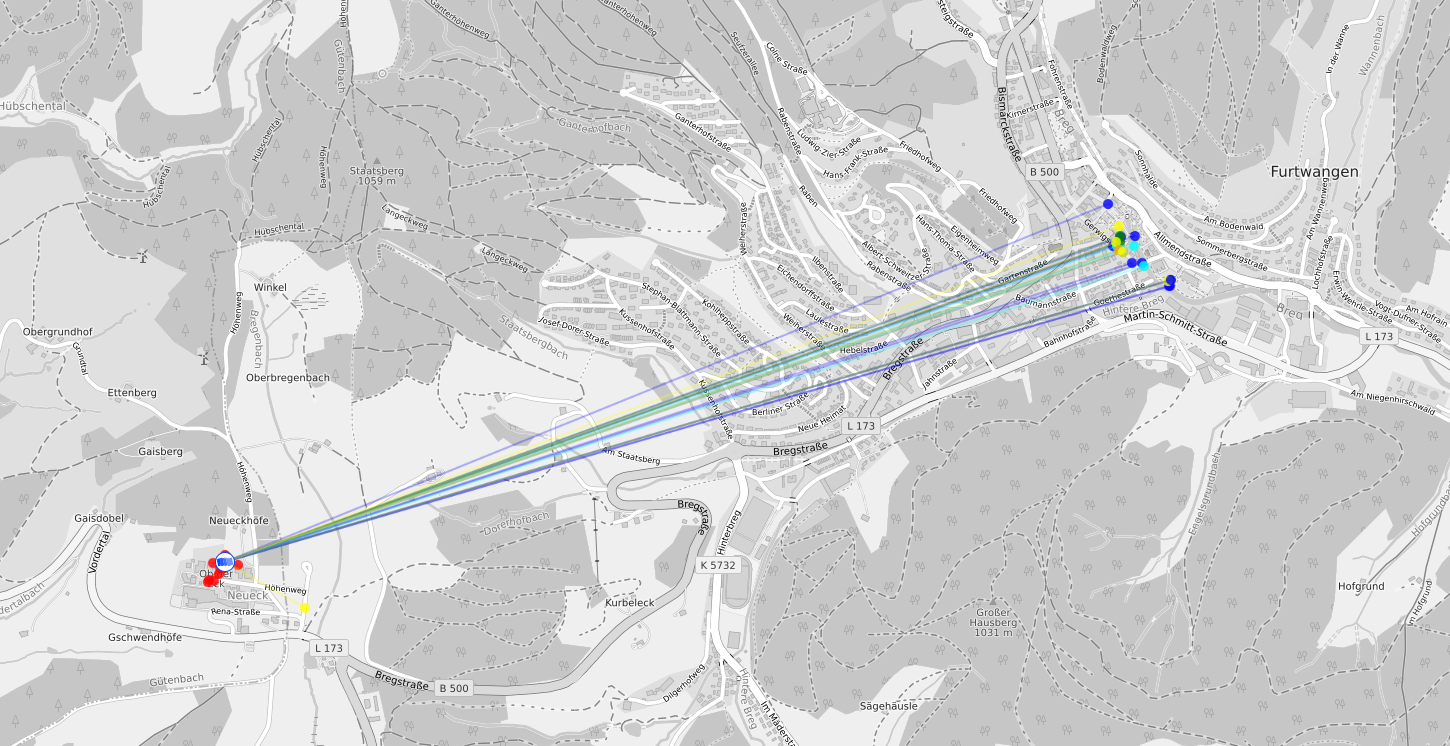
\includegraphics[width=0.9\textwidth]{pictures/ttn-mapper/moved_gateway_example.png}
    \caption[Example of false data being displayed on a \acl{TTNM} map due to a gateway being moved]{
        Screenshot of a \ac{TTNM} map showing an example of false data being displayed due to a gateway being moved.
        The gateway placed on the right is the one on the roof of the DL0FIS clubhouse.
        The data points on the right are from before the gateway was moved there when it was still on the roof of the \ac{HFU} B building~\cite{ttn_mapper_ttn_2023}.
    }\label{pic:gateway-moved-example}
\end{figure}

\Cref{pic:gateway-moved-example} shows an example where this happened in \ac{TTNM}.
It shows a gateway that was located on the \ac{HFU} B building, but was then moved to its final location, the roof of the DL0FIS clubhouse.

\ac{TTNM} is supposed to perform a similar data cleaning as was described earlier based on the section ``My results were showing on the map before, but is gone now.'' in their FAQ~\cite{ttn_mapper_faq_nodate}.
However, as far as the duration of this thesis is concerned, this was not observed, as evidenced by \Cref{pic:gateway-moved-example}.

\ac{TTNL} could be improved by adding a feature to the \ac{TTNL} backend.
If a gateway moves further than a certain distance, each associated TtnMapperDatapoint having a timestamp before the relocation should be deleted to avoid the usage of false data in the calculations.

\subsubsection{Remove dependency on \acl{TTNM}}

Since this thesis is largely based on \ac{TTNM}, it would be beneficial to remove the dependency on it.
The \ac{TTNL} software would no longer be able to function in its current state if \ac{TTNM} was discontinued.
A glimpse of such a scenario was already encountered during development, when the \ac{TTNM} \ac{API} was offline for several hours on some days.

To remove the dependency on \ac{TTNM}, the \ac{TTNL} software could be extended to include its own \ac{REST} endpoints similar to \ac{TTNM}, providing the same ability to receive data directly from \ac{TTN}.
This would enable the \ac{TTNL} software to function without \ac{TTNM} and would also allow for more flexibility in data collection in the future.

\subsubsection{Better sharing of type definitions between Frontend and Backend}\label{subsubsec:outlook-sharing-type-definitions}

Because the frontend and backend were separated into two distinct repositories, certain \ac{TS} type definitions had to be duplicated across the two.
This resulted in some manual work when changing the type definitions, as changes had to be applied to both repositories.
In the future, this could be improved in several ways.
For example, the frontend and backend could be merged into a single repository, called a monorepo~\cite{narwhal_technologies_inc_monorepo_2022}.

The type definitions could also be moved to a separate repository that is used as a dependency in both the frontend and backend repositories.

\subsubsection{Choice of technologies}

This section will critically reflect on the choice of technologies used in this thesis as well as mention some alternatives.

\paragraph{Docker and Docker Compose}

The usage of Docker and Docker Compose was a good choice.
While it required extra effort to integrate the backend and frontend in a Docker Compose environment, the end result was worthwhile.
It made setting up a development environment on a \ac{VM} provided by the \ac{HFU} effortless.
The only addition that needed to be made manually was adding a Traefik reverse proxy to allow for secure \ac{HTTPS} connections to the frontend and backend services from outside the \ac{HFU} network~\cite{traefik_labs_traefik_2023}.

Using Docker and Docker Compose also allows for easy reproducibility of the project, as the Docker Compose stack also includes the PostGIS \ac{DB} and can be started with a single command.

\paragraph{Full Stack Frameworks (SvelteKit, Nuxt.js)}

As an alternative to the approach described in \Cref{subsubsec:outlook-sharing-type-definitions}, the entire project could have been written using a full-stack framework such as SvelteKit or Nuxt.js.
This would also have allowed the entire project to be in a single repository, which would have made sharing type definitions easier.

However, this would also have meant a much tighter coupling of the \ac{TTNL} frontend and backend.
As a result, it would no longer be possible to deploy the \ac{TTNL} frontend and backend services separately as Docker containers, since the entire project would have to be deployed as a single Docker container.

\paragraph{Prisma}

While Prisma enables the developer to write type safe \ac{DB} queries using \ac{TS}, it does not support all possible queries (yet).
Some advanced queries, such as the PostGIS one shown in \Cref{lst:sql-remove-outliers}, had to be written ``by hand'' using \ac{SQL} and executed using Prisma's \lstinline|$executeRaw| method.
There were several such cases in this thesis, which is why it might have been more suitable to not use Prisma at all and instead use \ac{SQL} in a more direct way.

However, Prisma's ability to generate migrations from a schema and its type safety justified its use.
Furthermore, the schema file of Prisma serves as indirect documentation for the \ac{DB} structure, which can be beneficial for other developers who wish to contribute to the project.

An alternative to Prisma would have been PgTyped, which is a library that can generate typesafe \ac{SQL} queries from \ac{TS} type definitions~\cite{salakh_pgtyped_2023}.

Another alternative would have been to use GraphQL instead of \ac{HTTP} \ac{REST} calls.
GraphQL is a method for writing \ac{API} queries that lets the client specify which data it wants to receive from the server~\cite{graphql_foundation_graphql_2023}.
It uses a syntax to modify and request data that is similar to \ac{JSON}.
In doing so, GraphQL also ships its own type system that can be used to generate type definitions for the frontend.

\subsection{Projects made possible due to better \acs{LoRaWAN} coverage in Furtwangen}

Now that there are several new \aclp{LRWGW} in Furtwangen, there are a number of projects that can be done in the future that would not have been possible before without installing such gateways by oneself.

This section will list some of these projects and describe how they could be implemented.

\subsubsection{Measuring the water level of the Breg river}

One of the \aclp{LRWED} ordered as part of this thesis is a Milesight EM310-UDL, an ultrasonic distance/level sensor.
As the \ac{LoRaWAN} network coverage of Furtwangen is now adequate for most outdoor \ac{LoRaWAN} sensor deployments, it would be possible to use this sensor to measure the water level of the Breg River flowing through the \ac{HFU} campus grounds.
This could allow for a prediction of the water level of the Breg River, which could in turn allow for a prediction of the water level of the Danube River, for example.
Installing this \acl{LRWED} as well as connecting it to \ac{TTN} and adding an \acf{AS} to it to allow monitoring of the water level of the Breg River would be a good future project for students of the \ac{HFU}, enabled by the \aclp{LRWGW} placed during this thesis.

\subsubsection{Measuring soil moisture and environmental conditions in the Furtwangen city park}

Also during the current semester, Samuel Kasper, a student of the \ac{DM} faculty of the \ac{HFU} wrote his bachelor's thesis on measuring the humidity and temperature of the soil to monitor plants and crop growth.
The installation of \aclp{LRWGW} in Furtwangen helped him in this regard, as he did not have to install his own \aclp{LRWGW} and instead could use the now existing infrastructure in the city.

\subsubsection{Monitoring of \acl{LRWGW}}

Another possible project would be an application that monitors the gateways and checks if they are still online.
Such a project could be realized with software like Node-RED~\cite{openjs_foundation_node-red_nodate}.
Alerting specific users if a gateway goes offline could also be implemented with Node-RED.

\subsection{Further research}

\subsubsection{Improving timestamp accuracy for \acl{ToA} geolocation method}

As mentioned in \Cref{subsec:conclusion-toa-tdoa}, the accuracy of the \ac{ToA} method could be greatly improved if nanosecond level timestamps were available.
Unfortunately, \ac{TTN} does not provide nanosecond level timestamps for the packets received by the \aclp{LRWGW}.
To solve this problem, a \ac{LNS} would need to be set up that has the ability to do that.

In addition, \aclp{LRWGW} would need to be time synchronized to achieve the best possible accuracy.
The latter problem could be solved by using \ac{GPS} receivers to time-synchronize the \aclp{LRWGW}.
While some \aclp{LRWGW} have built-in \ac{GPS} receivers, most do not.
For example, the Dragino DLOS8N that was used twice during this thesis has a \ac{GPS} built-in receiver~\cite{dragino_technology_co_ltd_dlos8n_2023}, but none of the others do.

Ultimately, using the \ac{ToA} method would require more specific hardware than what most of the \ac{TTN} community network currently uses.
This makes it unsuitable for widespread use on that particular network.

\subsubsection{Using \acl{ML} to improve the fingerprinting method}

There are several \ac{ML} methods that could be used to improve the fingerprinting method.

For example, \ac{kNN} could be used to determine the location of a \acl{ED} based on the \ac{RSS} values of the surrounding \aclp{LRWGW}.
\ac{kNN} also uses a \ac{DB} of fingerprints.
However, it does not calculate the center of the matching data points but uses the ``k nearest neighbors'' to determine the location of a \acl{ED}~\cite{anagnostopoulos_reproducible_2019}.

As was mentioned in \Cref{sec:related-work}, Perković et al.\ published a paper on the topic of \ac{LoRa}-based indoor localization where they used a deep learning approach.
They trained their network with \ac{RSS} values and position samples similar to the ones used in this thesis~\cite{perkovic_machine_2023}.

A multi-dimensional regression could be performed to enable the multilateration approach by including \ac{SNR} and \ac{SF} values.
This could improve the accuracy of the multilateration method while only requiring some training data per gateway to be collected.

\subsubsection{Gateway on the roof of the \acl{HFU} O building}

As was mentioned in \Cref{subsec:conclusion-hfu-o-building}, the roof of the O building would make another good location for a \acl{LRWGW}.
The permission by the building's owner was granted.
The problem that would need to be solved is getting a network connection as well as power to the roof of the building.

Another option that would only require getting power to the roof is to use a \acl{LRWGW} that has a \ac{LTE} backhaul connection.
However, getting a \ac{PoE} connection to the roof of the building would still be preferable due to its stability.

\subsubsection{Meshing / repeating of \aclp{LRWGW}}

While \ac{LoRa} allows for communication between any sort of \ac{LoRa} device, be it \acl{ED} or gateway, \ac{LoRaWAN} does not.
Theoretically, a gateway to gateway communcation in pure \ac{LoRa} is possible~\cite{dwijaksara_multihop_2019}.
However, this behavior is not implemented in the \ac{LoRaWAN} protocol.

If this functionality could be implemented in the \ac{LoRaWAN} protocol, it would allow for a sort of meshed network of \aclp{LRWGW}.
Gateways acting as repeaters in such a network could forward \ac{LoRaWAN} packets without the need for a backhaul connection as mentioned in \Cref{sec:gateways}.
Since the \ac{LoRaWAN} protocol doesn't provide this functionality yet, it would need to be tested with a custom implementation of gateway firmware first.

A \ac{LoRaWAN} related project that also uses \ac{LoRa} and can do meshing between \aclp{LRED} is Meshtastic~\cite{meshtastic_llc_meshtastic_2023}.
It uses hardware similar to the \aclp{LRWED} used in this thesis to create a meshed network of \aclp{LRED} that can communicate without the need for Internet access.

The German company Dryad Networks GmbH uses meshed \aclp{LRGW} to build a network that can be used with their products~\cite{dryad_networks_gmbh_silvanet_2023}.
It is utilized for the early detection of wildfires via a network of \ac{LoRa} sensors transmitting their information over meshed \aclp{LRWGW}.
This eliminates the requirement for a backhaul connection for every \aclp{LRWGW} spread throughout extensive forested regions.

Anton Petrov is going to write his master thesis about this topic in the coming winter semester of 2023/2024.
His thesis will also be supervised by Prof. Dr. Richard Zahoransky.

\subsubsection{Self-hosting of \acl{TTS} or ChirpStack}

Another interesting project would be to self-host an instance of a \ac{LNS} like \ac{TTS} or ChirpStack on \ac{HFU} infrastructure.
This would give students the opportunity to learn more about the inner workings of a \ac{LNS} and would also give the \ac{HFU} the ability to exert more control over the data collected by the \ac{LNS}.
Both of them are \ac{OSS} and can be self-hosted using Docker or Docker Compose.

\subsection{Privacy concerns}

Since the work in this thesis has shown that it is possible, at least at a rough level, to locate \aclp{LRWED} even without a \ac{GPS} receiver, there are some privacy concerns that need to be addressed.

\aclp{LRWED} are small and can be hidden easily while having a long battery life and long range.
This means that such devices could be used to track people without their knowledge over long periods of time even when not having access to \ac{GNSS} at all as long as there are enough \aclp{LRWGW} around to perform a rough multilateration or fingerprinting.

As \Cref{subsec:factory-building-of-the-e-wehrle-company} showed, it is also possible to roughly locate a \acl{LRWGW} with enough data collection and time.
This could allow bad actors to physically attack \aclp{LRWGW} connected to the public \ac{TTN} network even if they do not a have a public location set.

\section{Conclusion}

This section will summarize the results of the work in this thesis and aims to answer the research questions posed in \Cref{sec:introduction-research-questions}.

This thesis deployed a full-stack application using \ac{LoRaWAN} technology, covering all aspects from hardware to software.
The procedure involved the installation of \aclp{LRWGW}, collecting data using \aclp{LRWED} and transmitting the data packets to \acl{TTNM} through the \ac{TTN} \acl{LNS}.
Following that, the data is displayed on a website deployed within a containerized environment, including a backend \ac{API} service and a \acl{DB}.

The viability of \ac{RSS}-based localization methods has been evaluated, and it has been shown that they can be used with some degree of accuracy.
Although the accuracy of these methods, particularly outdoors, is lower than that of \ac{GNSS}, it is still sufficient for various uses, such as geofencing and others.
The low power consumption of \ac{LoRaWAN} makes it a viable option for battery-powered devices that do not need to be located with high accuracy.

Overall, the fingerprinting approach exhibited superior accuracy results; however, it requires a substantial amount of manual data collection work.
By contrast, the multilateration approach is simpler to implement and use as it doesn't require much manual work; nonetheless, its performance is highly susceptible to environmental factors.

The impact of environmental factors such as \ac{MPP} has proven to be significant.
It impacted all \ac{RSS}-based measurements, and somewhat affected the \ac{GNSS} measurements, as well.

In summary, this thesis implemented a complete \ac{LoRaWAN} application and evaluated \ac{RSS}-based localization methods for a range of practical applications.
The fingerprinting approach demonstrated higher precision through manual data collection.
However, the simpler multilateration approach proved to be susceptible to environmental factors, highlighting the potential of \ac{LoRaWAN} for energy-efficient location solutions.